%19/02 - Modesto
\chapter{Modelado de proteínas en la era de Alphafold}
\section{La historia del modelado de estructuras de proteínas contada por un concurso (CASP)}
Cada dos años, desde 1994, grupos del campo de la bioinformática estructural llevan a cabo un experimento mundial en el que predicen un conjunto de estructuras proteicas desconocidas en una competición controlada, similar a una prueba a ciegas, y comparan sus resultados con las estructuras obtenidas experimentalmente. Se trata del CASP (Critical assessment of Protein Structure Prediction).

Los mejores grupos de investigación del sector ponen a prueba sus nuevos métodos y protocolos en el CASP. Sin embargo, en el CASP13 (2018), una empresa de IA llamada Deepmind (filial de Google) entró en escena. Su método, llamado Alphafold ganó claramente el CASP13. Alphafold (v.1) implementó mejoras en algunos enfoques utilizados recientemente y creó un proceso completamente nuevo. En lugar de crear mapas de contactos a partir del alineamiento y luego plegar la estructura, utilizaron una unidad MRF (Markov Random Field) para extraer las características principales de la secuencia y el MSA por adelantado y procesar toda esta información en una red neuronal multicapa (llamada ResNet) que también predijo probabilidades de distancia en lugar de contactos, lo que dio como resultado una gran precisión. A continuación, Alphafold utiliza toda la información posiblemente obtenida para crear la estructura y luego mejorarla mediante la minimización de la energía (método de descenso más pronunciado) y la sustitución de porciones con una base de datos seleccionada de fragmentos de proteínas.

\begin{figure}[h]
\centering
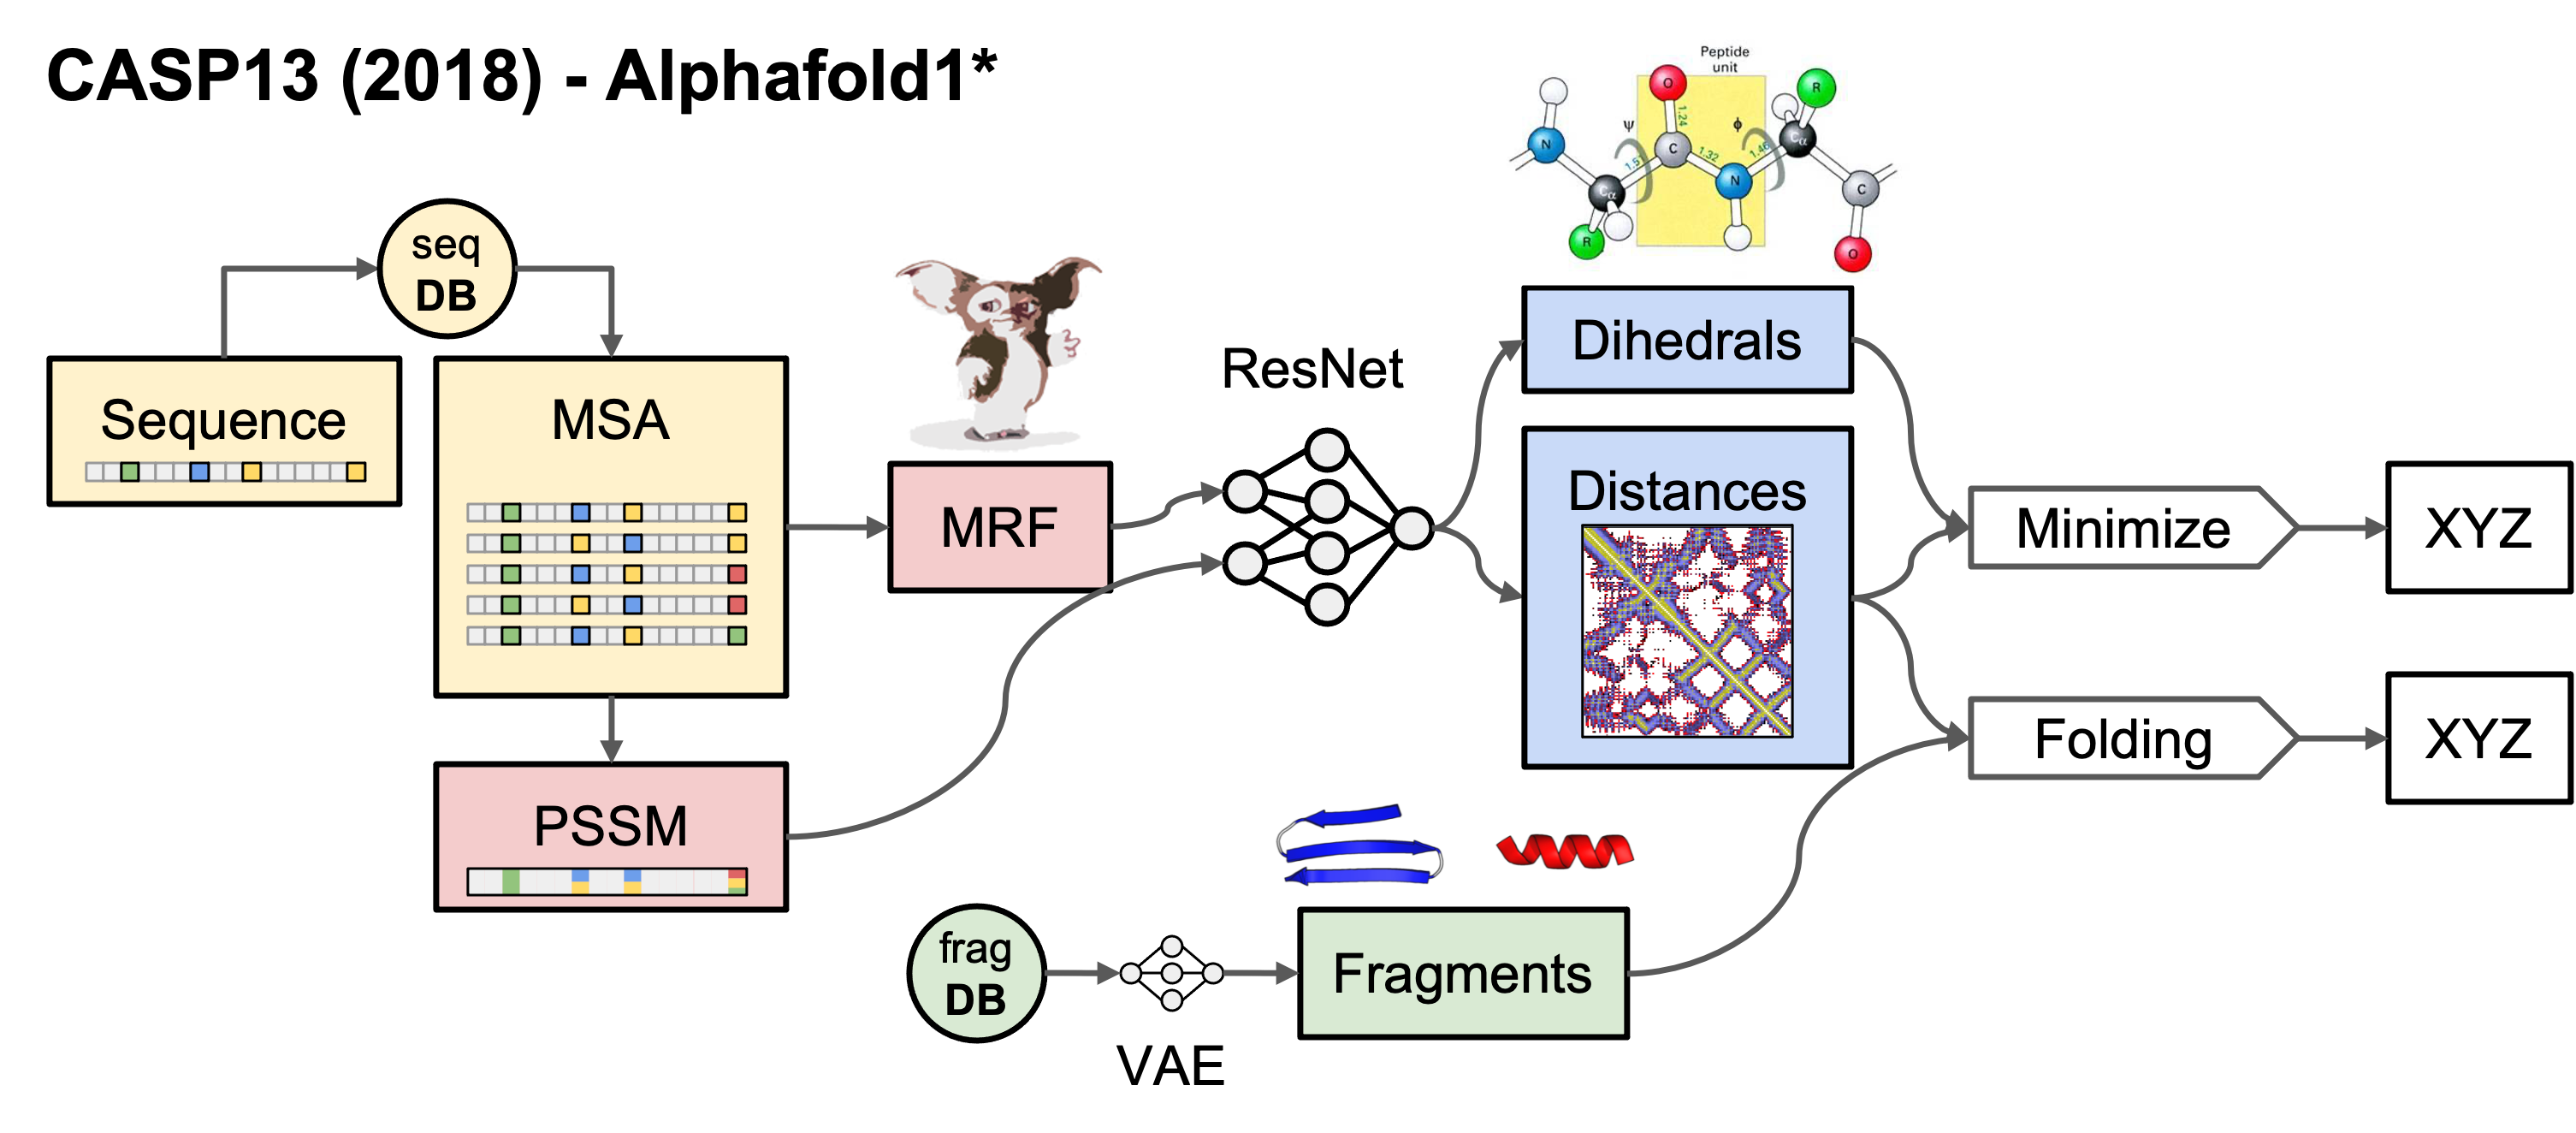
\includegraphics[width = 0.8\textwidth]{figs/alphafold1.png}
\caption{Flujo de trabajo del primer método Alphafold presentado en CASP13. MSA significa alineación múltiple de secuencias; PSSM indica Position-specific-scoring matrix y MRF significa Markov Random Field (o modelo Potts).}
\end{figure}

Después de Alphafold, también se desarrollaron métodos similares y se pusieron a disposición del público en general, como el trRosetta, del laboratorio Baker, disponible en el software de código abierto Rosetta y en el servidor Robetta. Esto llevó a cierta controversia (sobre todo en Twitter) sobre el acceso abierto al software CASP y más tarde DeepMind publica todo el código en GitHub.

\section{CASP14 o cuando la predicción de la estructura de las proteínas alcanza la mayoría de edad para los biólogos (no estructurales)}
Había mucho revuelo en CASP14 y los chicos de DeepMind no decepcionaron a nadie. Alphafold2 dejó muy atrás a todos sus competidores, tanto en términos relativos (puntuación frente a los demás grupos) como en términos absolutos (RMSD alfa-carbono más bajo). Como se ha destacado anteriormente, la precisión de muchas de las estructuras predichas estaba dentro del margen de error de los métodos de determinación experimental.

\begin{figure}[h]
\centering
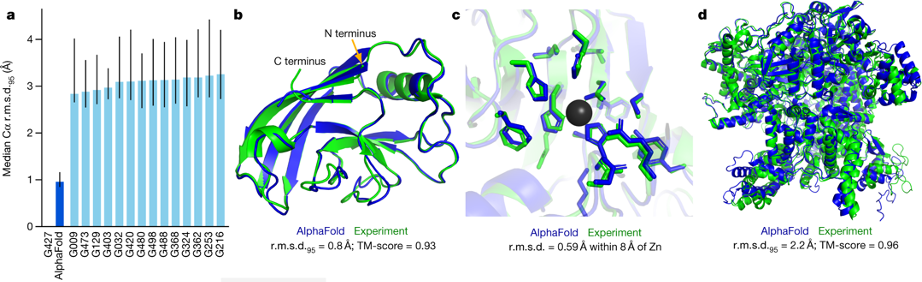
\includegraphics[width = 0.8\textwidth]{figs/jumper2021.png}
\caption{Rendimiento de Alphafold2 en el conjunto de datos CASP14 en relación con las 15 mejores entradas. Los datos son la mediana y el intervalo de confianza del 95\% de la mediana, para RMSD alfa-carbono. Los paneles b-c-d muestran ejemplos de comparación entre el modelo y las estructuras experimentales.}
\end{figure}

Deepming tardó algún tiempo (ocho meses, lo que hoy en día es una eternidad) en publicar el método y liberar el código en Github, pero otros métodos nuevos, como RoseTTAfold y C-I-Tasser fueron capaces de obtener resultados similares y estaban disponibles en servidores públicos, lo que quizá empujó a Deepmind a ponerlo todo a disposición de la comunidad científica. No es de extrañar que un grupo de científicos independientes (Sergey Ovchinnikov, Milot Mirdita y Martin Steinegger) decidieran implementar Alphafold2 en un cuaderno Colab, llamado ColabFold, que está disponible gratuitamente en línea a través de la plataforma de cuadernos Colab de Google. Otras implementaciones libres de Alphafold han estado y están disponibles, pero ColabFold ha sido la más ampliamente discutida y conocida. Implementaron algunos trucos para acelerar el modelado, sobre todo el uso de MMSeqs2 (desarrollado por el grupo de Martin Steinegger) para buscar estructuras homólogas en Uniref30, lo que convirtió a Colabfold en un método rápido que hizo casi inútiles todos los métodos avanzados anteriores. Este fue el verdadero avance en el campo de la predicción de estructuras de proteínas, haciendo accesible Alphafold y, también muy importante, facilitó el desarrollo posterior del método, implementando muy rápidamente nuevas características, como la predicción de complejos de proteínas, que de hecho se mencionó por primera vez en Twitter y luego dio lugar a varios nuevos métodos dedicados, incluyendo AlphaFold-multimer de Deepmind o AlphaPullDown.

\section{Alphafold como paradigma de una nueva era}
\subsection{¿Por qué Alphafold es tan preciso?}
La filosofía detrás de Alphafold v.2 (a partir de ahora, sólo Alphafold) y métodos relacionados es tratar el problema del plegamiento de proteínas como un problema de aprendizaje automático, similar al procesamiento de imágenes. En todos estos problemas, la entrada al modelo de aprendizaje profundo es un volumen (tensor 3D). En el caso de la visión por ordenador, las imágenes 2D se expanden como volúmenes debido a los canales RGB o HSV. Del mismo modo, en el caso de la predicción de distancias, las características 1D y 2D predichas se transforman y empaquetan en un volumen 3D con muchos canales de información entre residuos.

\begin{figure}[h]
\centering
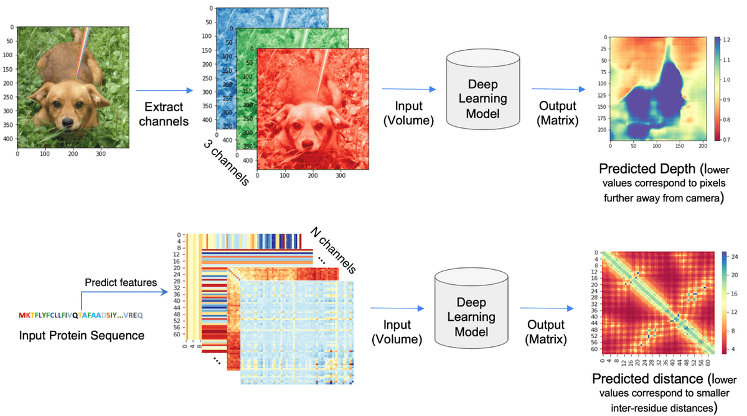
\includegraphics[width = 0.8\textwidth]{figs/machine_fold.png}
\caption{Desde la perspectiva del desarrollo de métodos de Deep Learning, el problema de la predicción del distograma de proteínas o distancia en valor real (fila inferior) es similar al «problema de predicción de profundidad» en visión por ordenador.}
\end{figure}

Alphafold puede explicarse como un pipeline con tres tareas interconectadas (véase la imagen inferior). En primer lugar, a diferencia de Alphafold v.1, la entrada de Alphafold es un MSA «en bruto», es decir, la red de aprendizaje profundo extrae la información coevolutiva directamente del MSA. Consulta varias bases de datos de secuencias de proteínas y construye un MSA que se utiliza para seleccionar plantillas. Esto puede ser un paso limitante que afecte a la velocidad del modelado (véase más adelante), pero también puede estar relacionado con la precisión del modelo, como se ha demostrado recientemente en CASP15.

En la segunda parte del diagrama, AlphaFold toma la alineación de secuencias múltiples y las plantillas, y las procesa en un \textbf{transformador}. Este proceso ha sido denominado por algunos autores como inter-residue interaction map-threading. El objetivo de esta parte es extraer capas de información para generar mapas de interacción de residuos. Un mejor modelo del MSA mejorará la caracterización de la geometría de la red, lo que simultáneamente ayudará a refinar el modelo del MSA. Es importante destacar que, en el AF2 Evoformer, este proceso es iterativo y la información va y viene por toda la red. En cada paso de reciclaje, la complejidad del mapa aumenta y, por tanto, el modelo mejora (el modelo original utiliza 3 ciclos). Como se explica en el post de Carlos Outerial en el sitio OPIG:
\begin{quote}
Esto es más fácil de entender con un ejemplo. Supongamos que observas el alineamiento múltiple de secuencias y notas una correlación entre un par de aminoácidos. Llamémoslos A y B. Usted parte de la hipótesis de que A y B están próximos, y traslada esta suposición a su modelo de la estructura. Posteriormente, examinas dicho modelo y observas que, puesto que A y B están próximos, hay muchas probabilidades de que C y D también lo estén. Esto conduce a otra hipótesis, basada en la estructura, que puede confirmarse buscando correlaciones entre C y D en el MSA. Repitiendo esto varias veces, se puede llegar a comprender bastante bien la estructura.
\end{quote}

La tercera parte del pipeline es el módulo de construcción de la estructura, que utiliza la información de los pasos anteriores para construir un modelo 3D de la estructura de la proteína de la secuencia de consulta. Esta red le dará un modelo único end-to-end, sin ningún paso de optimización de la energía. La construcción del modelo se basa en un nuevo concepto de generación de estructuras 3D, denominado \textbf{IPA (Invariant Point Attention)} y en el uso de una lista curada de ángulos de torsión parametrizados para generar las cadenas laterales. Los intentos anteriores de desarrollar un método de extremo a extremo no tuvieron éxito porque la representación de la estructura no era óptima. Incluso los métodos implementados después de AlphaFold, como RoseTTAFold, utilizan métodos menos eficientes y a menudo predicen muy rápidamente y con precisión las coordenadas de la columna vertebral, pero requieren programas externos para generar un modelo de todos los átomos.

\begin{figure}[h]
\centering
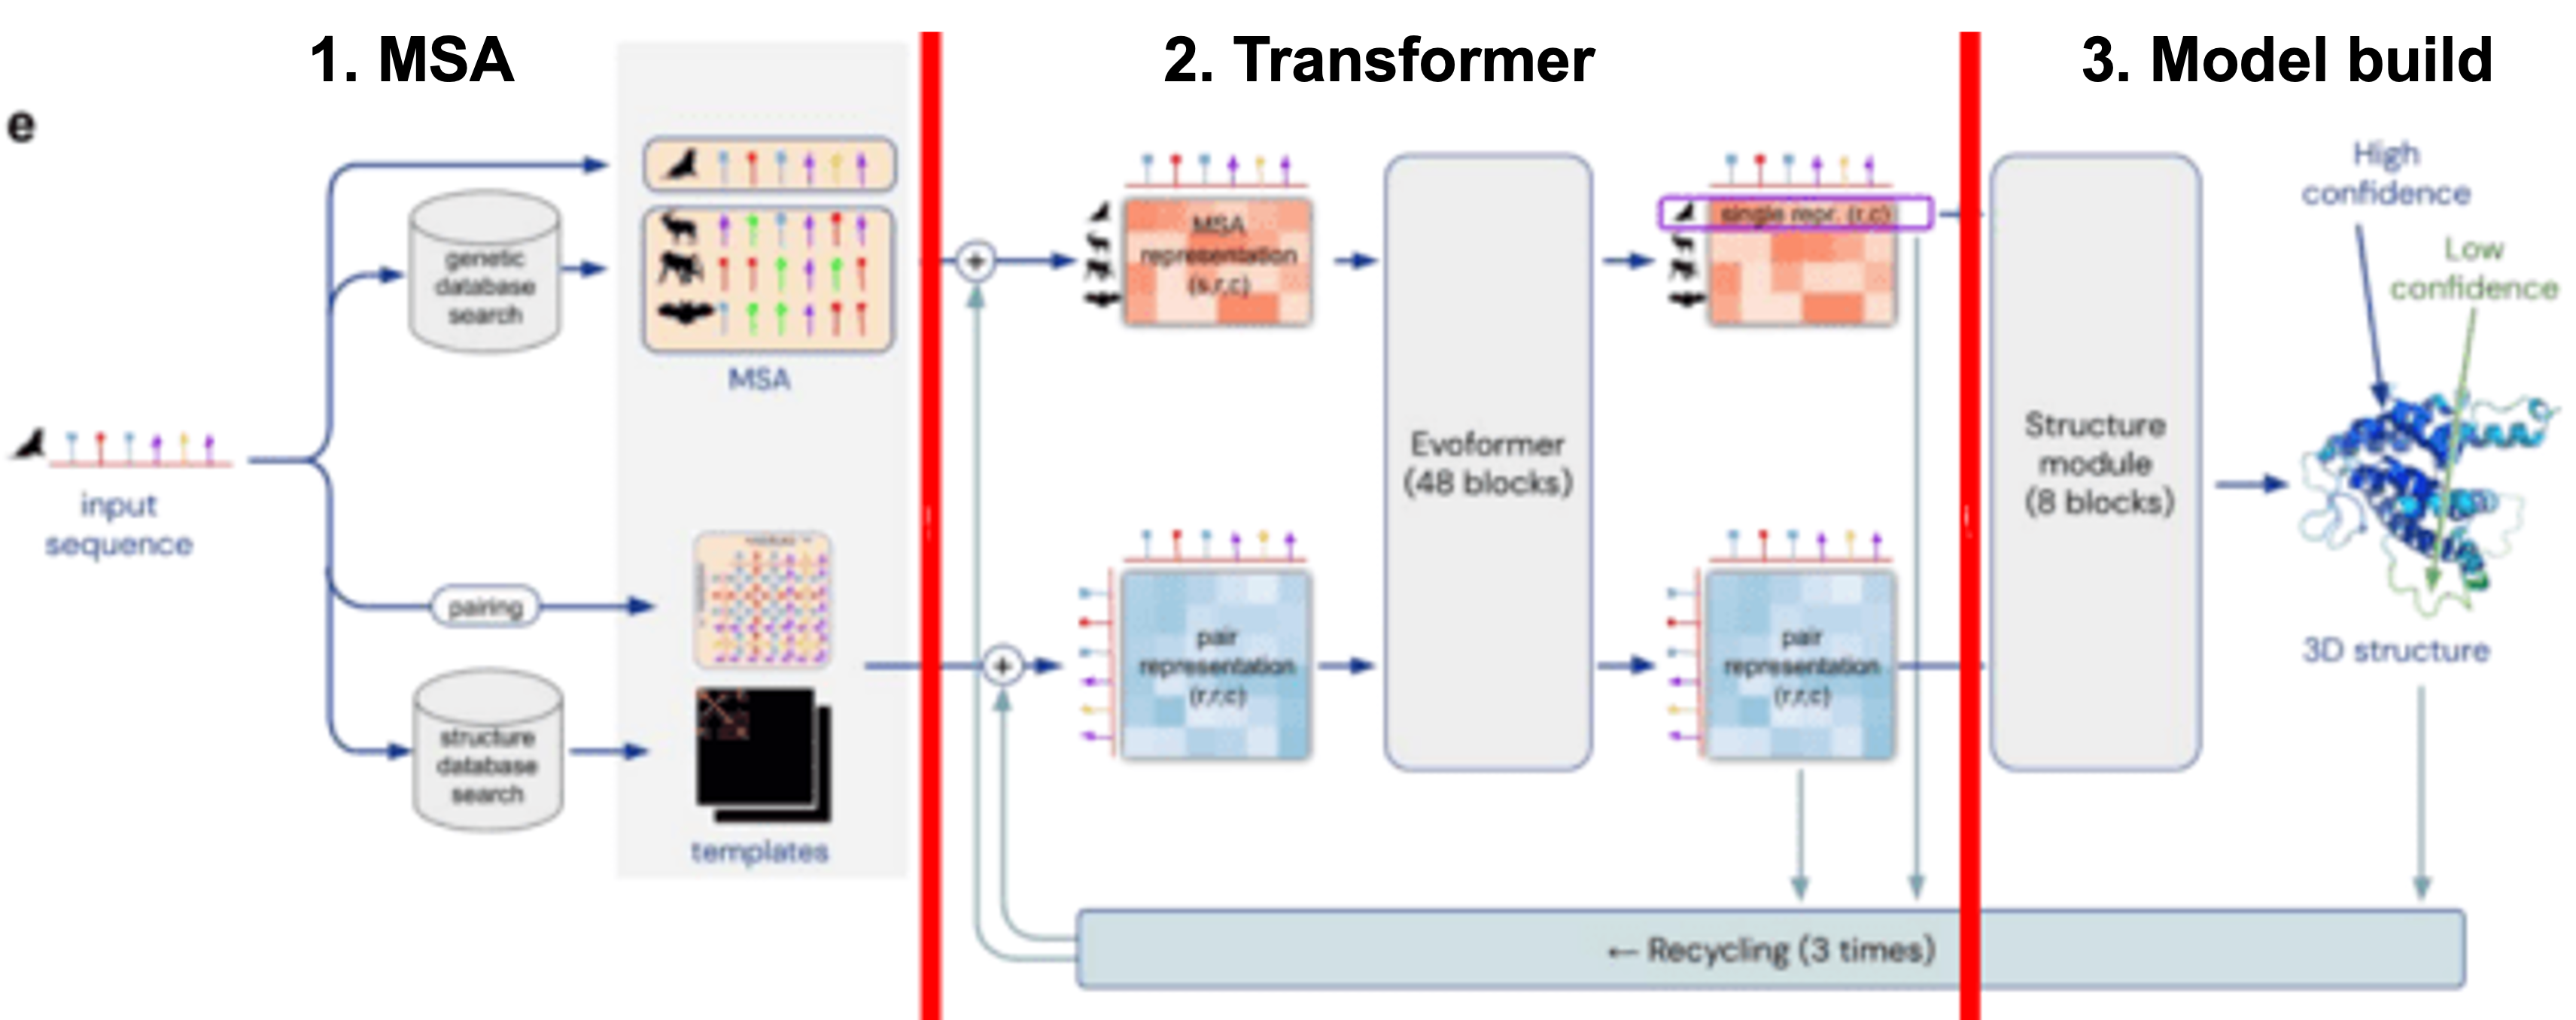
\includegraphics[width = 0.8\textwidth]{figs/alphafold2.png}
\end{figure}

Como para la mayoría de los métodos anteriores, Alphafold dará mejores resultados con proteínas con estructuras relacionadas conocidas y con muchos homólogos en las bases de datos Uniref. Sin embargo, comparado con nada, probablemente dará resultados útiles (limitados) para el llamado «genoma oscuro». Para un trabajo con fagos y elementos móviles bacterianos, secuenciar eso es a menudo frustrante, ya que más del 50\% de las proteínas no tienen homólogos en la base de datos. Así que tenemos un montón de proteínas de función desconocida... Sin embargo, como sabemos que la estructura está más conservada que la secuencia, podemos utilizar la estructura para averiguar la función de nuestras proteínas oscuras. Hay algunos recursos para esto, como los servidores FoldSeek y Dali. Se puede subir el archivo PDB del modelo y buscar estructuras relacionadas en la base de datos RCSB PDB y también en la base de datos Alphafold.

Como ya se ha mencionado, Colabfold pretende agilizar el proceso utilizando MMSeqs en el primer bloque. Además, también se puede adaptar el número de pasos de reciclado. Además, se han desarrollado (y evolucionado) diferentes cuadernos Colabfold para permitir cierta personalización y otras características, como el procesamiento por lotes de múltiples proteínas evitando la recompilación y la identificación de interacciones proteína-proteína.

Los modelos Alphafold pueden evaluarse mediante la \textbf{pLDDT} media, una métrica de confianza por residuo. Se almacena en los campos del factor B de los archivos mmCIF y PDB disponibles para su descarga (aunque a diferencia del factor B, un pLDDT más alto es mejor). La confianza del modelo puede variar mucho a lo largo de una cadena, por lo que es importante consultar la confianza al interpretar las características estructurales. Muy a menudo, los fragmentos de menor confianza no son producto de una mala predicción, sino un indicador de desorden de la proteína.

Otra medida es el PAE (predicted aligned error). Es el error previsto en $\AA$ entre cada par de residuos. Esto no tiene en cuenta ninguna estructura «verdadera», sino que es el error predicho. Así, los bloques de bajo PAE en la matriz PAE muestran que la posición relativa de todos esos residuos es segura, lo que puede mostrar, por ejemplo, que esos residuos forman un dominio bien plegado. pLDDT es un tipo diferente de predicción de error. En lugar de ser la predicción del error por pares entre dos residuos, pLDDT es básicamente «cuánta confianza tengo en la predicción de la posición de cada residuo». En ambos casos, estos valores son devueltos por el modelo de predicción y son estimaciones

Alphafold también se asoció con EMBL-EBI y Uniprot y generó una enorme base de datos curada de proteínas de organismos modelo, la base de datos Alphafold. Esta base de datos aumentó del 48\% al 76\% la fracción del proteoma humano con datos estructurales, y también significa grandes aumentos en el caso de otros organismos modelo, como, incluyendo microorganismos y plantas.

\subsection{¿Ahora qué? La era post-Alphafold}
Como ya se ha mencionado, RoseTTAFold se publicó al mismo tiempo que el artículo y el código de AlphaFold, aunque está claramente inspirado en las capacidades de AlphaFold en CASP14. Se basa en una red de tres pistas, y las implementaciones recientes han permitido predecir interacciones de proteínas con ácidos nucleicos. Otros métodos como AlphaFold y RoseTTAFold se lanzaron posteriormente, al igual que OpenFold y UniFold, que se basan en el marco PyTorch Transformers AI. Más recientemente, RoseTTAFold2, que extiende la arquitectura de tres pistas sobre toda la red e incorpora otros nuevos avances y trucos de AlphaFold, como el FAPE (frame aligned point error) o pasos de reciclado durante el entrenamiento, dando lugar a un modelo de extremo a extremo equivalente en precisión a AF2 para monómeros y AF2-multimer para complejos, con mejor escalado computacional en proteínas y complejos mayores de 1000 residuos.

El uso de MSA se ha citado como una limitación para AlphaFold y métodos relacionados. Sin embargo, las predicciones son significativamente peores sin MSA o con MSA sin profundidad. Una forma de mejorar las predicciones es utilizar un modelo de lenguaje natural de proteínas (PLN), es decir, un modelo entrenado para predecir secuencia a secuencia y que no dependa de buenos MSA. Omegafold y ESMfold (también en Colabfold) son dos nuevas implementaciones que sólo requieren una única secuencia. Son bastante rápidas y funcionan mejor que AlphaFold cuando se utiliza una única secuencia. Sin embargo, dado que PLN se entrena con secuencias existentes, estos métodos obtienen resultados significativamente peores con secuencias huérfanas. Es decir, los modelos lingüísticos parecen limitarse a recordar los MSA de entrenamiento.

La aparición de ESMfold y del Atlas Metagenómico complementario se vio como un nuevo paso que podría desencadenar una nueva revolución en el campo, ya que fue desarrollado por científicos de META. Así que ahora se trataba de una especie de batalla entre Google y Facebook por los métodos de IA más potentes para el modelado de proteínas. Sin embargo, el verano pasado supimos que META había decidido interrumpir el proyecto ESM.

AlphaFold se utilizó de alguna forma en más de la mitad de los protocolos, y aunque el método AlphaFold estándar funcionó mejor que muchos otros métodos, varios grupos lograron mejoras significativas para proteínas monoméricas y ensamblajes de proteínas. En resumen, aprendimos en CASP15 que hay dos formas principales de mejorar AlphaFold: (1) un uso más eficiente de las plantillas, aumentando el tamaño de la base de datos o el muestreo a través de MSA más eficientes, o (2) hackear AlphaFold para utilizar dropouts para generar miles de modelos para cada objetivo, lo que aumenta el tiempo computacional pero también aumenta las posibilidades de obtener mejores modelos. Se han propuesto otras pequeñas mejoras, como pasos de refinamiento o el uso de una búsqueda de plantillas mejorada o nuevas capacidades de puntuación basadas en superficies de Voronoi o Deep Learning.

\subsection{Corolario: ¿Resolvió Deepmind la paradoja de Levinthal?}
El desarrollo de Alphafold y de la base de datos de estructuras Alphafold en colaboración con el EMBL-EBI ha sido el origen de una nueva era. Además, en un nuevo giro, el Atlas Metagenómico de Meta AI descubre prácticamente todo el espacio proteico. Gracias a estos hitos se ha incrementado enormemente la cobertura del espacio de estructuras proteicas, lo que prácticamente cierra la brecha secuencia-estructura. Desde 2020, muchas publicaciones y revistas científicas de todo el mundo publicaron largos artículos sobre el significado de este gran avance en la ciencia y sus aplicaciones en biotecnología y biomedicina y DeepMind afirmó haber resuelto un Gran Desafío de 50 años en bioquímica.

En otras palabras, después de AlphaFold, ¿ya no sería necesario realizar cristalografía de rayos X o resonancia magnética nuclear? En primer lugar, los modelos AlphaFold pueden utilizarse en mapas de densidad electrónica y ayudar a resolver casos complejos. Así, el nuevo marco ayuda a los cristalógrafos a centrar su trabajo en las estructuras más difíciles y sin resolver, como las espirales o las holoproteínas, que provocan modulaciones y desafíos en el desarrollo de los métodos cristalográficos.

Sin embargo, algunos científicos sostienen que Alphafold2 y RoseTTAfold en realidad hacen trampa, ya que no resuelven realmente el problema, sino que generan una vía de aprendizaje profundo que es capaz de eludir el problema. De acuerdo con esto, se ha demostrado que los métodos de aprendizaje automático en realidad no reproducen las rutas de plegamiento esperadas mientras que mejoran las estructuras durante los pasos de reciclaje.

En conclusión, la paradoja de Levinthal no está (todavía) totalmente resuelta, aunque parece estar cerca. Prácticamente, está resuelta para la mayor parte del espacio proteico, pero si una proteína no tiene un homólogo en las bases de datos, todavía quedarán algunas preguntas abiertas.

\section{Limitaciones de Alphafold}
Entre las limitaciones se encuentran problemas con complejos de proteínas con otras moléculas como ADN, regiones desordenadas, variantes de splicing alternativo y falta de información evolutiva. El problema del splicing es muy importante en biomedicina. No hay estructuras en PDB de prácticamente ninguna variante de splicing, por lo que no se pueden predecir y puede ser un problema para mutantes específicos de las proteínas o diagnóstico de enfermedades raras. 

Un ejemplo de un target difícil es la proteína Bam35 de un bacteriófago. Se trata de una proteína SSB (single-stranded binding) con un OB-fold. Suelen formar multímeros a la hora de unirse al ADN. Esta proteína tenía unos valores de GMQE mut bajo, con una identidad también reducida. Se crearon tres modelos distintos y se vio que en los tres había una región conservada y una región diversa. La región conservada se utilizó para comparar frente a las bases de datos, pudiendo encontrar casos de similitudes. 

\section{Alphafold 3}
Alphafold v3 (mayo 2024) ha permitido modelar estructuras de proteínas en relación con otras estructuras como ADN y ARN. Esto es muy importante para el diseño de fármacos. El código está accesible, pero tiene muchas limitaciones. 